%%%%% 例題17（18.2 光の屈折 の末尾）＝ 原本【例題20】〈屈折の法則〉 %%%%%%%%%%
% 問題文・KEY は原本（p117）からの転写．原本の（指針）欄は空欄，解答も載っていないので
% 指針・解答はこちらで書き起こした（他章の例題と同じ扱い）．
\begin{reidaiunit}
\begin{reidai}{屈折の法則}
\begin{zuright}{54mm}
\hspace{1zw}水面から深さ$h\U{m}$のところに沈んだ物体$\mathrm{A}$を外から観察するとき，物体は本来ある場所よりも少し浮いた位置$\mathrm{B}$にあるように見える．これは，実際には境界面で光が屈折するために図のような経路で目に光が入ってくるが，人間の感覚では光が境界面で直進するように錯覚するため，$\mathrm{B}$点から光が来ているように見えるからである．

\hspace{1zw}物体$\mathrm{A}$を水面のほぼ真上から見る場合について以下の問に答えよ．ただし水の屈折率を$n$，空気の屈折率を1とする．
\zusep
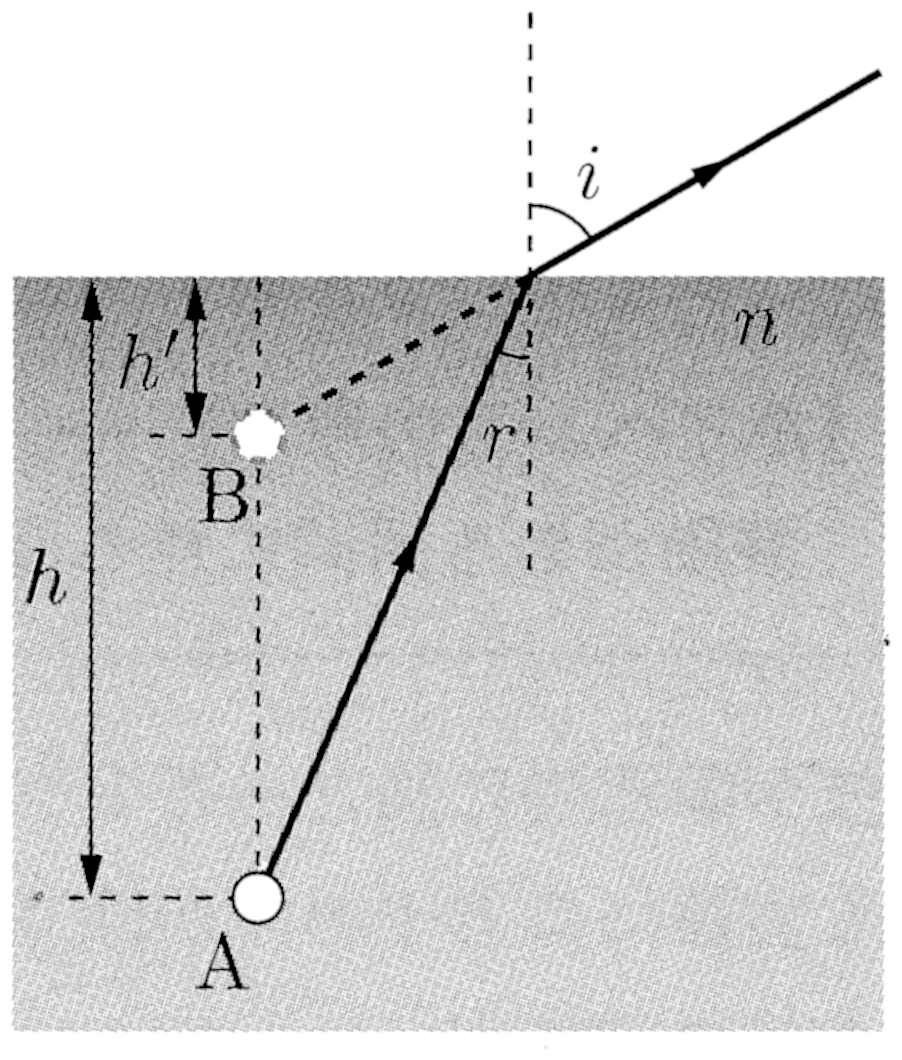
\includegraphics[keepaspectratio,width=54mm]{fig/ch18_ex_apparent.png}
\end{zuright}
\begin{komon}
\ko{1} 図において，$i$, $r$の間に成り立つ屈折の法則を$n$を用いて示せ．
\ko{2} 物体$\mathrm{A}$の見かけの深さ$h^\prime\U{m}$を，$h$, $i$, $r$を用いて表せ．
\ko{3} ほぼ真上から見る，すなわち$i$, $r$が非常に微小な角であることを用いて$h^\prime$を$n$, $h$で表せ．
\end{komon}
\end{reidai}

\begin{sisinE}
まず{\gtfamily 光がどちら向きに進んでいるかを確認する}．光は水中の$\mathrm{A}$から出て水面で屈折し，空気中の目に入る．したがって{\gtfamily 入射角は水中側の$r$，屈折角は空気側の$i$}である（図の文字の割り当てが$i$＝空気側であることに注意）．

見かけの位置$\mathrm{B}$は，{\gtfamily 目に入ってくる屈折光をそのまま逆向きにまっすぐ延長した直線}と，$\mathrm{A}$を通る鉛直線との交点である．人間は光が折れ曲がったことを知らずに，来た方向にまっすぐ物体があると感じるからである．

(2)は，水面上の屈折点を$\mathrm{P}$，$\mathrm{A}$の真上の水面上の点を$\mathrm{O}$とおき，{\gtfamily 同じ長さ$\overline{\mathrm{OP}}$を2通りに表す}のが要点．$\mathrm{A}$から見れば$\overline{\mathrm{OP}}=h\tan r$，$\mathrm{B}$から見れば$\overline{\mathrm{OP}}=h^\prime\tan i$である．

(3)は$|\theta|\ll 1$のとき$\tan\theta\fallingdotseq\sin\theta$が使えることを利用する．
\end{sisinE}

\Key{屈折の法則 $n_1\sin i=n_2\sin r$．見かけの位置は「屈折光を逆に延長した先」．}

\begin{kaitou}
\begin{komon}
\ko{1} 光は水中から空気中へ進むので，入射角が$r$，屈折角が$i$である．水の屈折率が$n$，空気の屈折率が1であるから，屈折の法則より
       \Ana{n\sin r=1\cdot\sin i\hspace{4mm}\text{すなわち}\hspace{4mm}n\sin r=\sin i\Ans}
\ko{2} 水面上の屈折点を$\mathrm{P}$，物体$\mathrm{A}$の真上にある水面上の点を$\mathrm{O}$とする．直角三角形$\mathrm{OPA}$に着目すると
       \Ana{\overline{\mathrm{OP}}=h\tan r}
       である．一方，目に届く屈折光を逆向きに延長した直線は$\mathrm{P}$で鉛直線と角$i$をなし，その延長線上の見かけの位置が$\mathrm{B}$であるから，直角三角形$\mathrm{OPB}$に着目すると
       \Ana{\overline{\mathrm{OP}}=h^\prime\tan i}
       である．この2式の左辺は同じ長さであるから，
       \Ana{h\tan r=h^\prime\tan i}
       よって，
       \Ana{h^\prime=h\frac{\tan r}{\tan i}\U{m}\Ans}
\ko{3} $i$, $r$がともに微小であるとき$\tan i\fallingdotseq\sin i$, $\tan r\fallingdotseq\sin r$と近似できるので，(2)の答えは
       \Ana{h^\prime\fallingdotseq h\frac{\sin r}{\sin i}}
       となる．ここで(1)の屈折の法則$n\sin r=\sin i$より$\dfrac{\sin r}{\sin i}=\dfrac{1}{n}$であるから，
       \Ana{h^\prime=\frac{h}{n}\U{m}\Ans}
\end{komon}
\end{kaitou}

\begin{chuu}
水の絶対屈折率は$n\fallingdotseq 1.33$であるから，$h^\prime\fallingdotseq 0.75h$となる．
つまり{\gtfamily 真上から見た水中の物体は，実際の深さの約$3/4$の位置に浮いて見える}．
プールの底が思ったより浅く見えるのはこのためである．なお$h^\prime$が$h$に比例するので，見かけの深さは「実際の深さの一定割合」になる．
\end{chuu}
\end{reidaiunit}
